\chapter{Opis projektnog zadatka}
		
		Cilj ovog projekta je izraditi web aplikaciju koja će 
		računovodstvenim tvrtkama ubrzati digitalizaciju. Glavna funkcionalnost aplikacije je detekcija dokumenta
		s učitanih slika i izrada OCR-a (optical character recognition) detektiranog teksta. Učitana slika mora biti slikana iz dobrog kuta te mora imati približno pravokutan oblik. Moguće je istovremeno učitati do 50 uslikanih dokumenata.
		
		Pristupanjem na aplikaciju korisniku se prikazuju opcije prijave ili registracije ovisno o tome ima li profil. Za prijavu je potrebna email adresa i šifra, a za registraciju  potrebno je upisati:
		\begin{packed_item}
			\item {ime}
			\item {prezime}
			\item {email adresa}
			\item {identifikacijski broj (dobiva se pri zaposlenju u tvrtku)}
			\item {željena šifra}
			\item {ponovno napisana šifra}
		\end{packed_item}
		
		Nakon prijave ovisno o ulozi se korisniku dodjeljuju prava. Svaki korisnik ima mogućnost učitati dokument. Nakon što je napravljen OCR dokumenta, korisniku se prikazuje sažetak dokumenta. Korisnik može skenirani dokument označiti kao točno skenirani ili kao krivo skenirani. Što god korisnik odabrao, dokument i korisnikov odabir spremaju se u bazu.	Korisnici aplikacije su zaposlenik, revizor, računovođa, direktor i administrator.
		
		\textit {Zaposlenik} ulaskom u aplikaciju odabire jednu od dvije mogućnosti može aplikacijom skenirati dokumente i može vidjeti povijest svih svojih skeniranja (datum i skenirani dokument). Nakon skeniranja željenog broja dokumenata, zaposleniku je prikazan sažetak svakog od priloženih dokumenata, te on provjerava ispravnost svakog pojedinačnog dokumenta. Odobreni dokumenti šalju se revizoru. 
		
		\textit{Revizor} dobiva dokumente koje mu šalju zaposlenici te ih provjerava sve kako bi svaki dokument preusmjerio do ispravnog računovođe zaduženog za taj tip dokumenata. Ako revizor skenira dokumente aplikacija će automatski iz dobivenog teksta odrediti kojem računovođi se šalje dokument.
		
		\textit{Računovođa} dobivene dokumente arhivira. Aplikacija prilikom arhiviranja	dokumentu dodjeljuje jedinstveni broj arhiva. Također, računovođa ima opciju slanja dokumenata direktoru na potpis prije arhiviranja. Računovođa može arhivirati poslane dokumente tek kada dobije potvrdu da je direktor potpisao traženi dokument.
		
		\textit {Direktor} može vidjeti povijest svih dokumenata te povijest i	statistike svih zaposlenika. Direktor ima mogućnost promaknuti članove tvrtke nakon čega će administratoru poslati obavijest u kojem se traži da se zaposleniku daju veće ovlasti u aplikaciji. Također, potpisuje dokumente koje mu šalje računovođa te ih prosljeđuje natrag nakon potpisa.
		
		\textit{Administrator} ima apsolutne ovlasti. Ima pristup bazi podataka skeniranih dokumenata i podacima zaposlenika te može davati veće ovlasti zaposlenicima po zahtjevu direktora.
		
		Postoje tri tipa dokumenata – računi, ponude i interni dokumenti. Računi će u
		svom tekstu nakon OCR-a imati oznaku računa koja je veliko slovo R te šest znamenaka, oznaka ponude će imat veliko slovo P i devet znamenaka, a oznaka internog dokumenta
		„INT“ i četiri znamenke. Računi osim oznake sadrže ime klijenta, artikle s cijenama i
		ukupnu cijenu. Ponude su kao računi, ali ne sadrže ime klijenta. Interni dokumenti
		sadrže samo nestrukturirani tekst.\\
		
		\eject
		
		\section{Primjeri u \LaTeX u}
		
		\textit{Ovo potpoglavlje izbrisati.}\\

		U nastavku se nalaze različiti primjeri kako koristiti osnovne funkcionalnosti \LaTeX a koje su potrebne za izradu dokumentacije. Za dodatnu pomoć obratiti se asistentu na projektu ili potražiti upute na sljedećim web sjedištima:
		\begin{itemize}
			\item Upute za izradu diplomskog rada u \LaTeX u - \url{https://www.fer.unizg.hr/_download/repository/LaTeX-upute.pdf}
			\item \LaTeX\ projekt - \url{https://www.latex-project.org/help/}
			\item StackExchange za Tex - \url{https://tex.stackexchange.com/}\\
		
		\end{itemize} 	


		
		\noindent \underbar{podcrtani tekst}, \textbf{podebljani tekst}, 	\textit{nagnuti tekst}\\
		\noindent \normalsize primjer \large primjer \Large primjer \LARGE {primjer} \huge {primjer} \Huge primjer \normalsize
				
		\begin{packed_item}
			
			\item  primjer
			\item  primjer
			\item  primjer
			\item[] \begin{packed_enum}
				\item primjer
				\item[] \begin{packed_enum}
					\item[1.a] primjer
					\item[b] primjer
				\end{packed_enum}
				\item primjer
			\end{packed_enum}
			
		\end{packed_item}
		
		\noindent primjer url-a: \url{https://www.fer.unizg.hr/predmet/proinz/projekt}
		
		\noindent posebni znakovi: \# \$ \% \& \{ \} \_ 
		$|$ $<$ $>$ 
		\^{} 
		\~{} 
		$\backslash$ 
		
		
		\begin{longtblr}[
			label=none,
			entry=none
			]{
				width = \textwidth,
				colspec={|X[8,l]|X[8, l]|X[16, l]|}, 
				rowhead = 1,
			} %definicija širine tablice, širine stupaca, poravnanje i broja redaka naslova tablice
			\hline \multicolumn{3}{|c|}{\textbf{naslov unutar tablice}}	 \\ \hline[3pt]
			\SetCell{LightGreen}IDKorisnik & INT	&  	Lorem ipsum dolor sit amet, consectetur adipiscing elit, sed do eiusmod  	\\ \hline
			korisnickoIme	& VARCHAR &   	\\ \hline 
			email & VARCHAR &   \\ \hline 
			ime & VARCHAR	&  		\\ \hline 
			\SetCell{LightBlue} primjer	& VARCHAR &   	\\ \hline 
		\end{longtblr}
		

		\begin{longtblr}[
				caption = {Naslov s referencom izvan tablice},
				entry = {Short Caption},
			]{
				width = \textwidth, 
				colspec = {|X[8,l]|X[8,l]|X[16,l]|}, 
				rowhead = 1,
			}
			\hline
			\SetCell{LightGreen}IDKorisnik & INT	&  	Lorem ipsum dolor sit amet, consectetur adipiscing elit, sed do eiusmod  	\\ \hline
			korisnickoIme	& VARCHAR &   	\\ \hline 
			email & VARCHAR &   \\ \hline 
			ime & VARCHAR	&  		\\ \hline 
			\SetCell{LightBlue} primjer	& VARCHAR &   	\\ \hline 
		\end{longtblr}
	


		
		
		%unos slike
		\begin{figure}[H]
			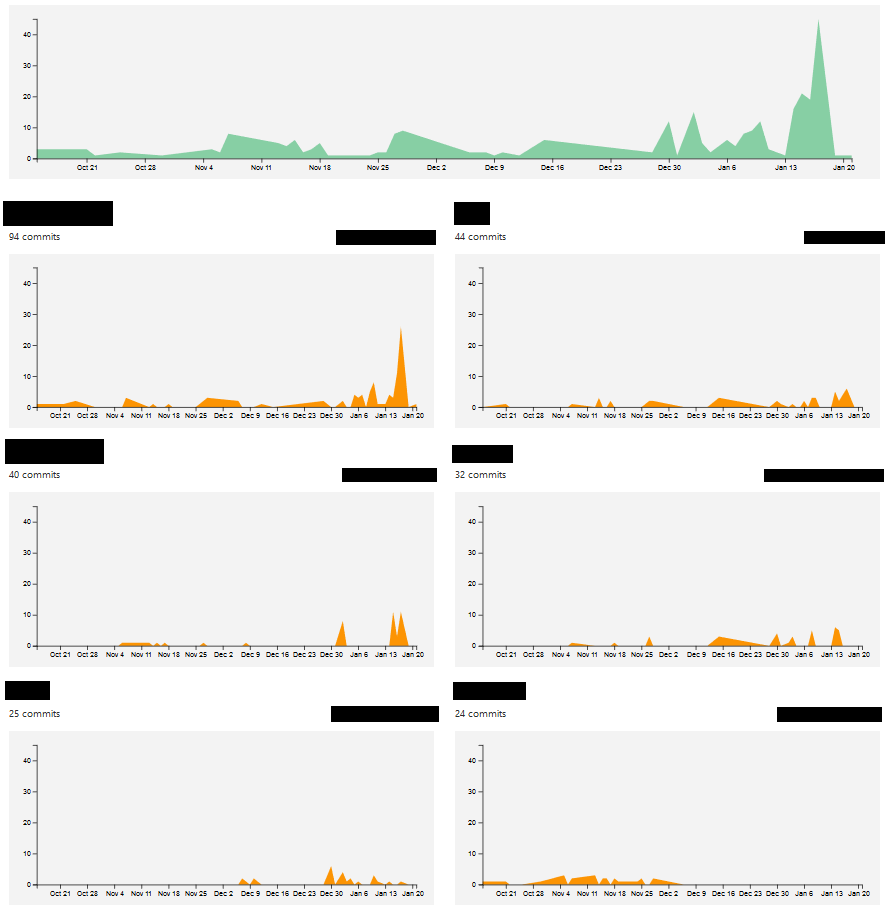
\includegraphics[scale=0.4]{slike/aktivnost.PNG} %veličina slike u odnosu na originalnu datoteku i pozicija slike
			\centering
			\caption{Primjer slike s potpisom}
			\label{fig:promjene}
		\end{figure}
		
		\begin{figure}[H]
			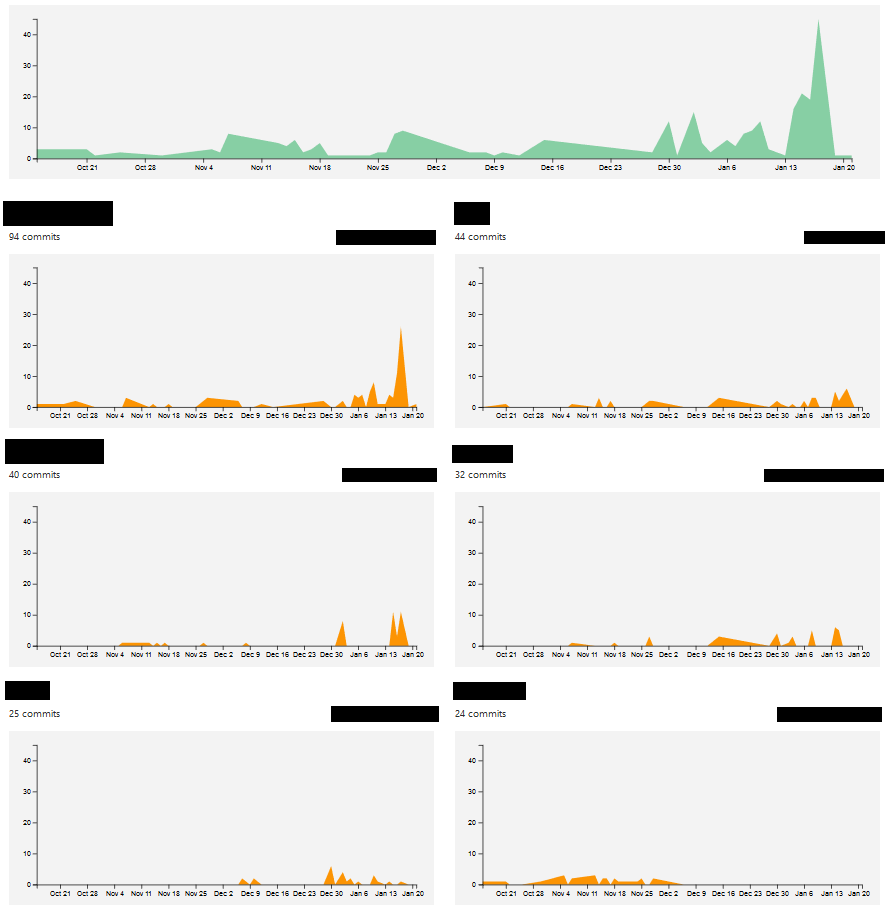
\includegraphics[width=\textwidth]{slike/aktivnost.PNG} %veličina u odnosu na širinu linije
			\caption{Primjer slike s potpisom 2}
			\label{fig:promjene2} %label mora biti drugaciji za svaku sliku
		\end{figure}
		
		Referenciranje slike \ref{fig:promjene2} u tekstu.
		
		\eject
		
	
